\begin{frame} \frametitle{The Block-chain database} 
	\begin{center}
		As database for new faces, we implemented a \textbf{Block-chain}. \\ 
		We used an open-source implementation of it, called 
		BigchainDB\footnote{Main page: {\color{red} 
		\url{https://www.bigchaindb.com}}. Documentation {\color{red}
		\href{http://docs.bigchaindb.com/projects/server/en/latest/introduction.html}
		{here}}.}. \\ We also used Docker\footnote{Main page: {\color{red} 
		\url{https://www.docker.com}}.} to deploy 4 containers running the
		application.
	\end{center}
	\vfill
	\begin{minipage}{.45\textwidth}
		\begin{figure}[H]
			
\includegraphics[width=.8\textwidth]{img/bchaindb}
		\end{figure}
	\end{minipage}
	\hfill
	\begin{minipage}{.45\textwidth}
		\begin{figure}[H]
			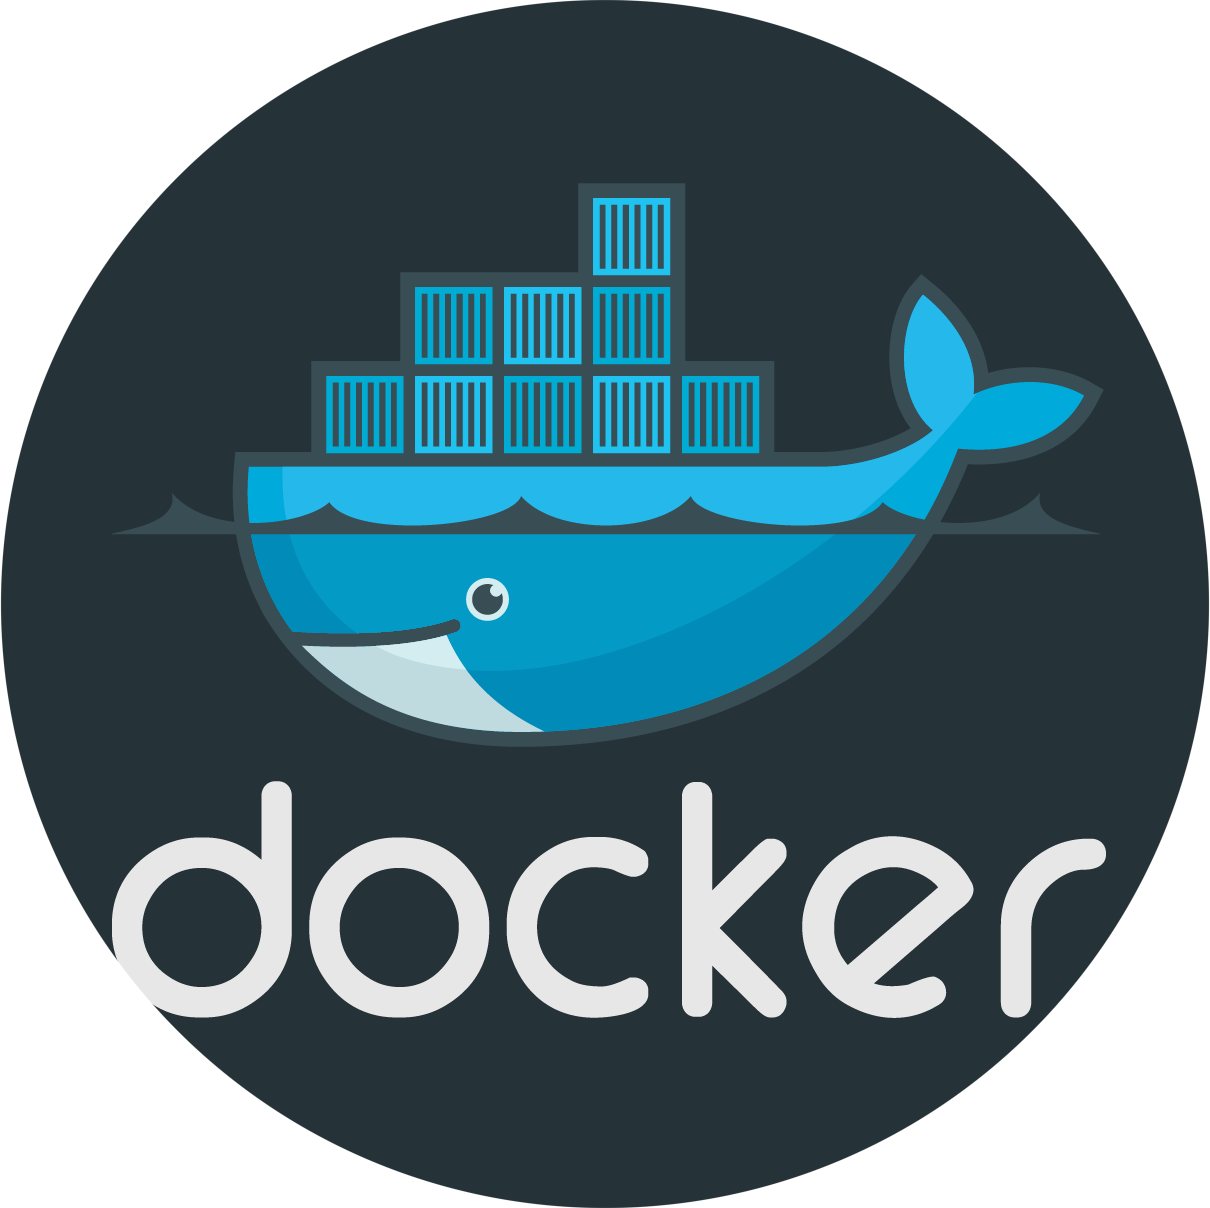
\includegraphics[width=.8\textwidth]{img/dockerlogo}
		\end{figure}
	\end{minipage}
	\vfill
\end{frame}
	
\begin{frame} \frametitle{Architecture Implementation}
	\centering \textbf{!!This is absolutely not meant for a real deployment!!}
	\begin{center} \scalebox{0.5}{ \begin{tikzpicture}[
		container/.style={rectangle, draw=black, fill=cyan!5 ,very thick, 
		minimum size=7.5em, align=center},
		ports/.style={draw=black, very thick, rectangle, rounded corners=2ex,
		minimum height=0.5in, minimum width=3in,align=center, rotate=90}
	]
		
		% Bigchaindb dockers
		\node[container, label={above:node1.casalinovalerio.com}] 
		(1) at (2,7) {Container: \\ \color{blue} Bigchain DB\#1};
		\node[container, label={above:node2.casalinovalerio.com}] 
		(2) at (7,7) {Container: \\ \color{blue} Bigchain DB\#2};
		\node[container, label={below:node3.casalinovalerio.com}] 
		(3) at (2,2) {Container: \\ \color{blue} Bigchain DB\#3};
		\node[container, label={below:node4.casalinovalerio.com}] 
		(4) at (7,2) {Container: \\ \color{blue} Bigchain DB\#4};
		
		% Nginx container
		\node[container] 
		(5) at (10.5,4.5) {Container: \\ \color{red} Nginx};
			
		% Ports
		\node[ports] (6) at (14,4.5) {Docker Ports};
		\node[ports] (7) at (18,4.5) {Server Ports};
			
		% Outline Boxes	
		\node(n1)[draw, blue, very thick, fit=(1)(2)(3)(4)(5)(6), 
		inner sep=2em, label={above:DOCKER SETUP}]{};
		\node(n2)[draw, brown, very thick, fit=(n1)(7),
		inner sep=2em,label={above:PHISICAL SERVER}]{};
			
		% Containers to Nginx	
		\draw[<->] (1.south) .. controls + (down:1em) .. ([yshift=0.5em]5.west);
		\draw[<->] (2.south) .. controls + (down:0.7em) .. ([yshift=1.5em]5.west);
		\draw[<->] (3.north) .. controls + (up:1em) .. ([yshift=-0.5em]5.west);
		\draw[<->] (4.north) .. controls + (up:0.7em) .. ([yshift=-1.5em]5.west);
	
		% Nginx to docker ports			
		\draw[line width=0.4em,<->,blue!30] (5.east) -- (6.north);
				
		% docker ports to server ports	
		\draw[ultra thick, red, <->] ([yshift=1.2in]6.south) -- 
		node[above]{\parbox[t]{2em}{22:22}} ([yshift=1.2in]7.north);
			
		\draw[ultra thick, red, <->] ([yshift=0.9in]6.south) -- 
		node[above]{\parbox[t]{2em}{80:80}} ([yshift=0.9in]7.north);
		
		\draw[ultra thick, red, <->] ([yshift=0.6in]6.south) -- 
		node[above]{\parbox[t]{3em}{443:443}} ([yshift=0.6in]7.north);
			
		\draw[ultra thick, red, <->] ([yshift=0.3in]6.south) -- 
		node[above]{\parbox[t]{4em}{9984:9984}} ([yshift=0.3in]7.north);
	
		\draw[ultra thick, red, <->] (6.south) -- 
		node[above]{\parbox[t]{4em}{9985:9985}} (7.north);
				
		\draw[ultra thick, red, <->] ([yshift=-0.3in]6.south) -- 
		node[above]{\parbox[t]{4em}{2812:2812}} ([yshift=-0.3in]7.north);
				
		\draw[ultra thick, red, <->] ([yshift=-0.6in]6.south) -- 
		node[above]{\parbox[t]{5em}{26656:26656}} ([yshift=-0.6in]7.north);
				
		\draw[ultra thick, red, <->] ([yshift=-0.9in]6.south) -- 
		node[above]{\parbox[t]{5em}{26657:26657}} ([yshift=-0.9in]7.north);
			
		\draw[ultra thick, red, <->] ([yshift=-1.2in]6.south) -- 
		node[above]{\parbox[t]{5em}{27017:27017}} ([yshift=-1.2in]7.north);
	\end{tikzpicture} }\end{center}
\end{frame}
		
\begin{frame} \frametitle{How to interact with the DB}
	We are assuming that we have an enstablished connection set up.
	\vfill
	\begin{block}{Query data}
		\texttt{connection.searchAssets('AwesomeAsset') \\
		.then(assets =$>$ console.log('Found assets:', assets))\\
		// Read the console to look at the assets}
	\end{block}
	\vfill
	\begin{block}{Load data (make a transaction)}
		\texttt{// Create transaction first (txTransferBob)				
		driver.Transaction.signTransaction(txTransferBob, alice.privateKey);	
		\\conn.postTransactionCommit(txTransferBobSigned);}
	\end{block}
	\vfill
	Simple as that...
\end{frame}